\subsubsection{Connessione dei nodi ai flussi di input}
\begin{figure} [H]
	\centering
	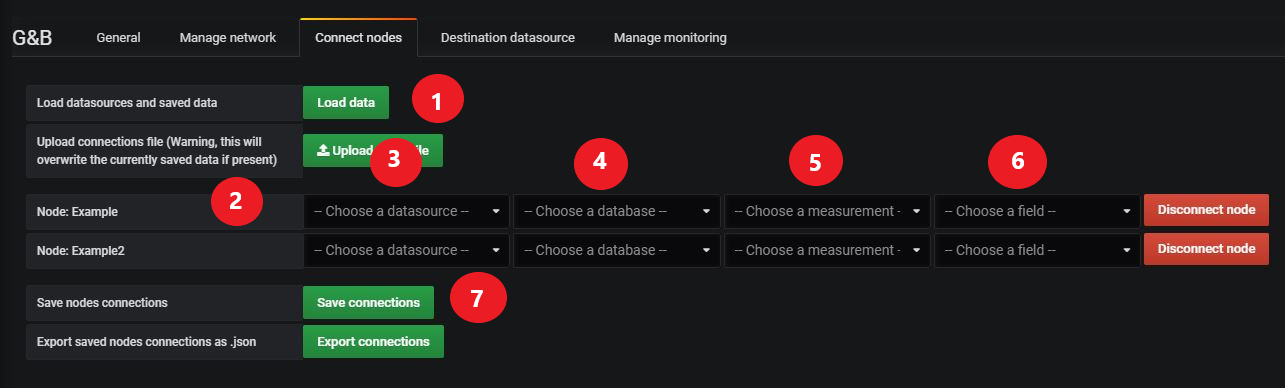
\includegraphics[scale=0.53]{Img/configurazionerete} 
	\caption{Tab di connessione} \label{} 
\end{figure} 
Dopo aver importato la rete Bayesiana tramite l'apposita tab, è possibile procedere alla configurazione delle connessioni per ogni nodo.
Il procedimento per connettere un nodo ad uno specifico flusso dati è il seguente:
\begin{enumerate}
	\item Cliccare sul pulsante \emph{"Load data"};
	\item Posizionarsi sulla riga del nodo del quale si vuole configurare il flusso di input;
	\item Scegliere la datasource nella quale è presente il flusso dati;
	\item Scegliere il database al quale appartiene il flusso dati;
	\item Scegliere la tabella (anche detta measurement in alcune datasource);
	\item Scegliere il campo specifico;
	\item Cliccare sul pulsante \emph{"Save connections"}.
\end{enumerate}
\subsubsection{Disconnessione dei nodi dai flussi di input}
\begin{enumerate}
	\item Cliccare sul pulsante \emph{"Load data"};
	\item Posizionarsi sulla riga del nodo del quale si vuole configurare il flusso di input;
	\item Cliccare sul pulsante \emph{"Disconnect node"};
	\item Cliccare sul pulsante \emph{"Save connections"}.
\end{enumerate}
\subsubsection{Esportazione della configurazione delle connessioni}
\begin{figure} [H]
	\centering
	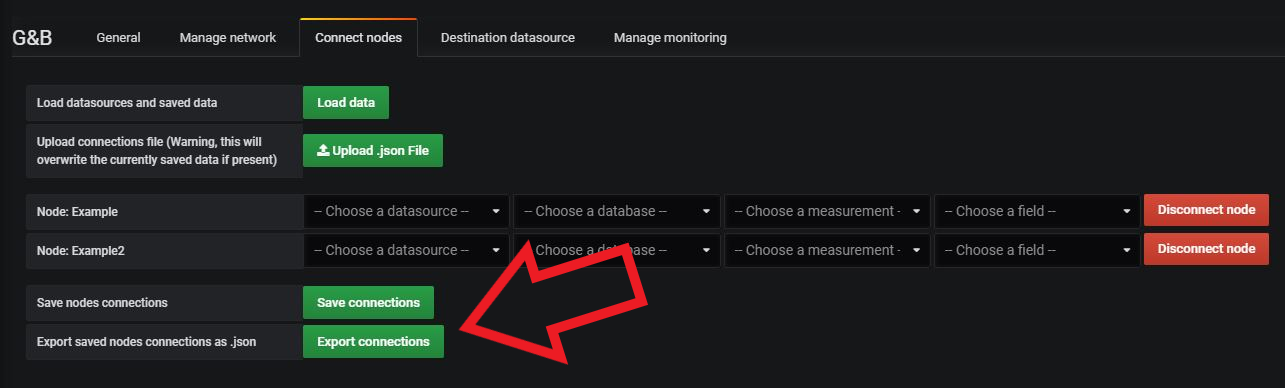
\includegraphics[scale=0.53]{Img/export} 
	\caption{pulsante \emph{"Export Connections"}} \label{} 
\end{figure} 
Per effettuare l'esportazione della configurazione delle connessioni cliccare sul pulsante \emph{"Export Connections"};
\subsubsection{Importazione della configurazione delle connessioni}
\begin{figure} [H]
	\centering
	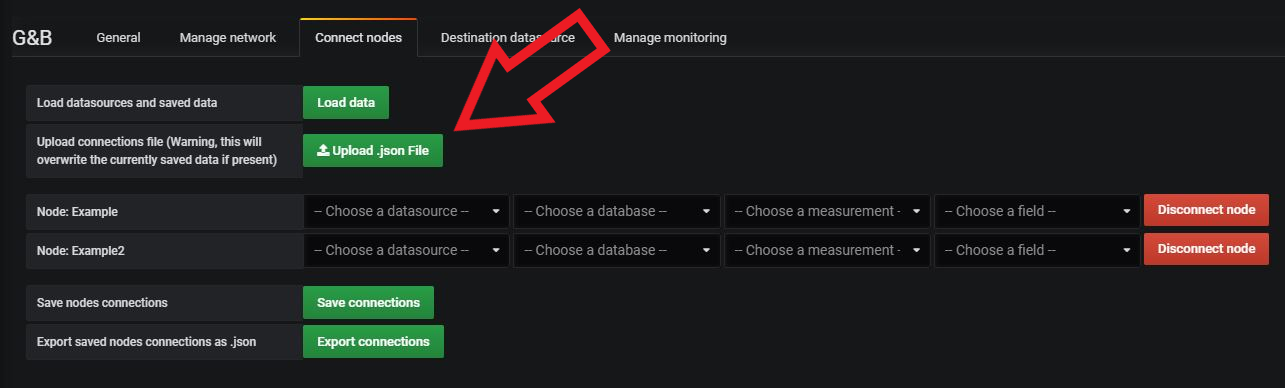
\includegraphics[scale=0.53]{Img/import} 
	\caption{pulsante \emph{"Import Connections"}} \label{} 
\end{figure} 
Per effettuare l'importazione della configurazione delle connessioni cliccare sul pulsante \emph{"Upload .json File"};